\chapter{Firm-growth statistics}
\label{chap:firmgrowth}

\section{Firm-growth statistics in the fluctuating state}
\label{sec:growing-observables}

We measure the two firm-growth facts on the relative sizes $S_i = N y_i$, whose
cross-sectional mean is one by construction. The common growth of the economy is divided
out in the same step, since $\ln S_i = \ln x_i - \ln M + \ln N$, so the size and its
growth $g_i = \Delta \ln S_i$ are the idiosyncratic part of a firm's trajectory, exactly
what the data measure. We follow the empirical protocol: each firm contributes while it
is listed, that is while $S_i$ stays above the immigration floor, and we read growth
rates over a fixed yearly horizon $\Delta t$ rather than the solver's adaptive one. All
statistics are taken in a late window, after the initial relaxation has passed, and
restricted to firms that persist across it.

Two cautions, detailed in Appendix~\ref{app:numerics}, shape the measurement: the
per-firm volatility is a mean-absolute-deviation estimator robust to the fat tails, and
the size--volatility relation is fitted only over its power-law range, the decline above
the small-firm plateau set by the immigration floor.

Figure~\ref{fig:growing-msb} shows both observables at the operating point
$\mu = -1.76$, $\sigma = 1.75$ marked in Figure~\ref{fig:phase-diagram}, in the
stationary fluctuating state. The size--volatility relation (left) now falls
monotonically over the fitted range, $\sigma(\bar S) \sim \bar S^{-\beta}$ with a clean
power law ($R^2 \approx 0.98$ in the economy shown), in contrast to the rising V of
Appendix~\ref{chap:results}: large firms are now less volatile than small ones, as in the
data. The growth-rate distribution (right) is
sharply peaked and fat-tailed, with both flanks heavier than the Laplace reference and
no systematic asymmetry between them. The two facts that the static critical model could
not deliver together, a monotone size--volatility decay and a symmetric fat-tailed tent,
are both present here, and both are stationary properties of the chaotic state rather
than transients of a relaxation.

\begin{figure}[htbp]
    \centering
    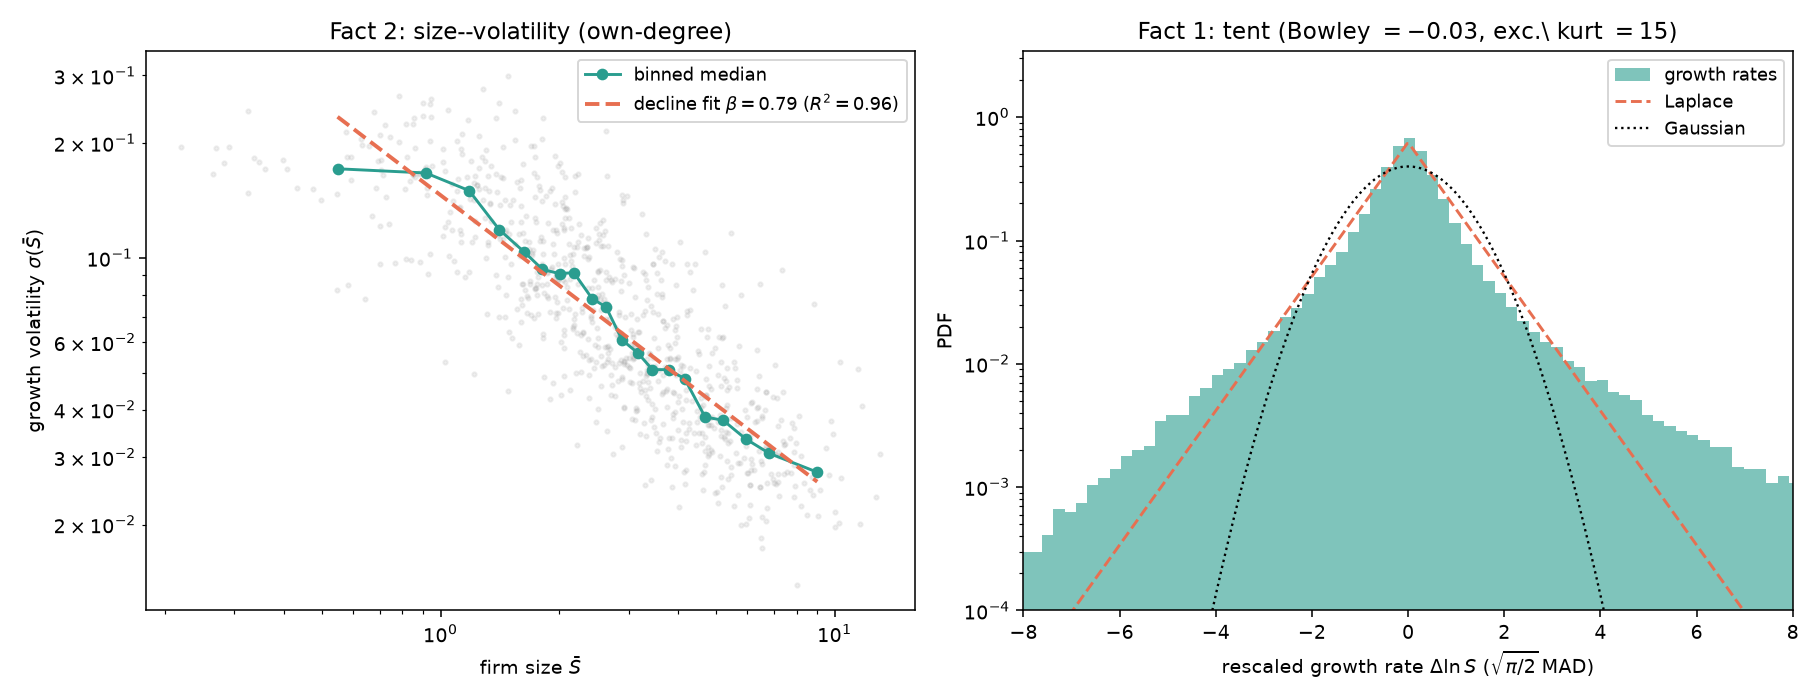
\includegraphics[width=\linewidth]{growing_stationary_msb.png}
    \caption{Firm-growth statistics at $\mu = -1.76$, $\sigma = 1.75$. Left: the
    size--volatility relation in a single economy ($N = 6400$) under the global mean-degree
    normalization; volatility falls as a
    power law over the fitted decline above the small-firm immigration-floor plateau
    (shaded), here with exponent $\beta \approx 0.5$ and $R^2 = 0.98$. Right: the
    growth-rate distribution pooled over economies, sharply peaked and fat-tailed,
    heavier than the Laplace reference on both flanks and close to symmetric
    (Bowley $\approx 0$), far above the Gaussian.}
    \label{fig:growing-msb}
\end{figure}

\section{Finite size and the mean-field limit}
\label{sec:growing-finite-size}

The chaotic state above is not equally robust at all system sizes, and the way it
strengthens with $N$ both validates the measurement and bears on the
size--variance exponent, which depends on the size of the economy rather than approaching
a fixed value. At small $N$ the persistent chaos is fragile: for many graph
realizations the shape, after fluctuating for a while, eventually collapses onto a fixed
point and freezes, recovering the relaxation transient of Appendix~\ref{chap:results}.
This is the known finite-size metastability of the fluctuating phase
\citep{roy2020}: rare large excursions drive firms below the floor, and the state can
fall into a frozen attractor. Figure~\ref{fig:growing-trajectories} contrasts the two
outcomes directly, a realization that freezes onto a fixed point against one that keeps
churning to the end of the run. Measuring in a short early window, as one is
tempted to do, reports the firms while they still fluctuate and so mistakes the frozen
transient for a stationary state; only integrating to long times separates the two.

\begin{figure}[htbp]
    \centering
    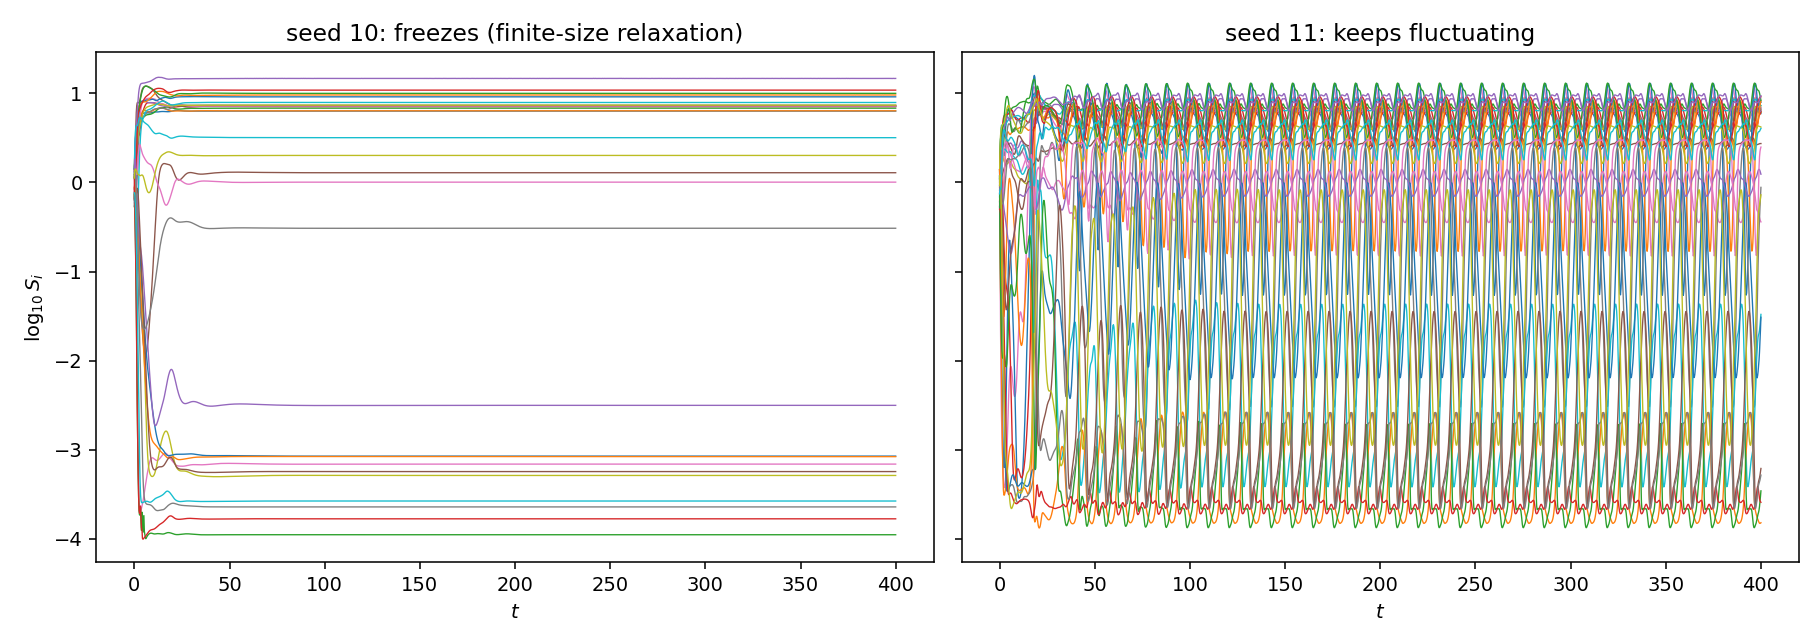
\includegraphics[width=\linewidth]{growing_trajectories.png}
    \caption{Two finite-size realizations at $N = 600$, $\mu = -1.76$, $\sigma = 1.75$.
    Left: the shares churn for a while and then freeze onto a fixed point, the
    finite-size relaxation transient. Right: a realization in which the chaos persists
    for the whole run. Whether a given realization freezes or keeps fluctuating is a
    finite-size accident that becomes rarer as $N$ grows.}
    \label{fig:growing-trajectories}
\end{figure}

Whether a realization freezes or keeps fluctuating is a finite-size accident that
becomes rarer as $N$ grows. The left panel of Figure~\ref{fig:growing-meanfield}
records the fraction of realizations that remain persistently chaotic at long times: it
is fragile at small $N$, with half to three-quarters of realizations persisting, and
reaches all of them by $N \approx 6000$. The fragility is
a finite-size effect; in the mean-field limit the fluctuating phase is the generic
outcome of the operating regime, consistent with the dynamical mean-field picture of
\citet{bunin2017} and \citet{roy2020}.

The size--variance exponent is a subtler matter, and turns on how the competition is
shared across the heterogeneous graph; its magnitude is the shallower of the two
comparisons we can make with the data. Under the global mean-degree normalization the exponent is not fixed by the mean-field limit:
measured on the persistent realizations it falls steadily and monotonically with system
size, from about $0.68$ at $N = 800$ toward $0.25$ at $N = 1.3\times10^4$
(Fig.~\ref{fig:growing-meanfield}, right), and it does not approach a nonzero constant.
There is no thermodynamic plateau to read off: an earlier fit of
$\beta(N) = \beta_\infty + c\,N^{-1/2}$ to an apparent intercept inside the band forced a
finite limit on a quantity that keeps falling, and rested in addition on a survivor
criterion that biases the measurement.

The exponent must instead be read at a finite economy size, because the data are, and on
the firm set the data actually use. We follow the empirical protocol: a firm is listed
while its size exceeds a fixed fraction of the mean firm and contributes growth rates only
while listed, keeping those with at least twenty such rates, as in the sample of
$15{,}788$ listed firms of \citet{moran2024}. Coexistence is then extensive, the
participation ratio $D_{\mathrm{eff}} = 1/\sum_i \bar w_i^2$ growing in proportion to $N$
and between $65$ and $78$ per cent of firms active at any time, in line with the $65$ per
cent of the empirical panel that enters the volatility estimate. The exponent on this
active set falls in the same way, and at the economy size for which the number of active
firms equals that sample, $N \approx 2\times10^4$, it is $\beta \approx 0.15$, at the
lower edge of the empirical band $0.15$--$0.20$ (Fig.~\ref{fig:growing-finite-economy}).
We read this as a finite-economy-size
effect rather than a thermodynamic exponent: real listed economies are finite, of order
$10^4$ firms, and the model reproduces the empirical exponent at that scale while
predicting a smaller one for a larger listed universe. The earlier impression of a
plateau inside the band, and the opposite worry of a collapse toward zero, were two faces
of one survivor artifact, since holding the delisting threshold fixed in share units while
the mean share falls as $1/N$ drops a growing fraction of firms through single transient
excursions; with delisting defined relative to the mean firm, as in the data, the active
population is extensive and the exponent sits at the empirical scale in the empirical
range.

\begin{figure}[htbp]
    \centering
    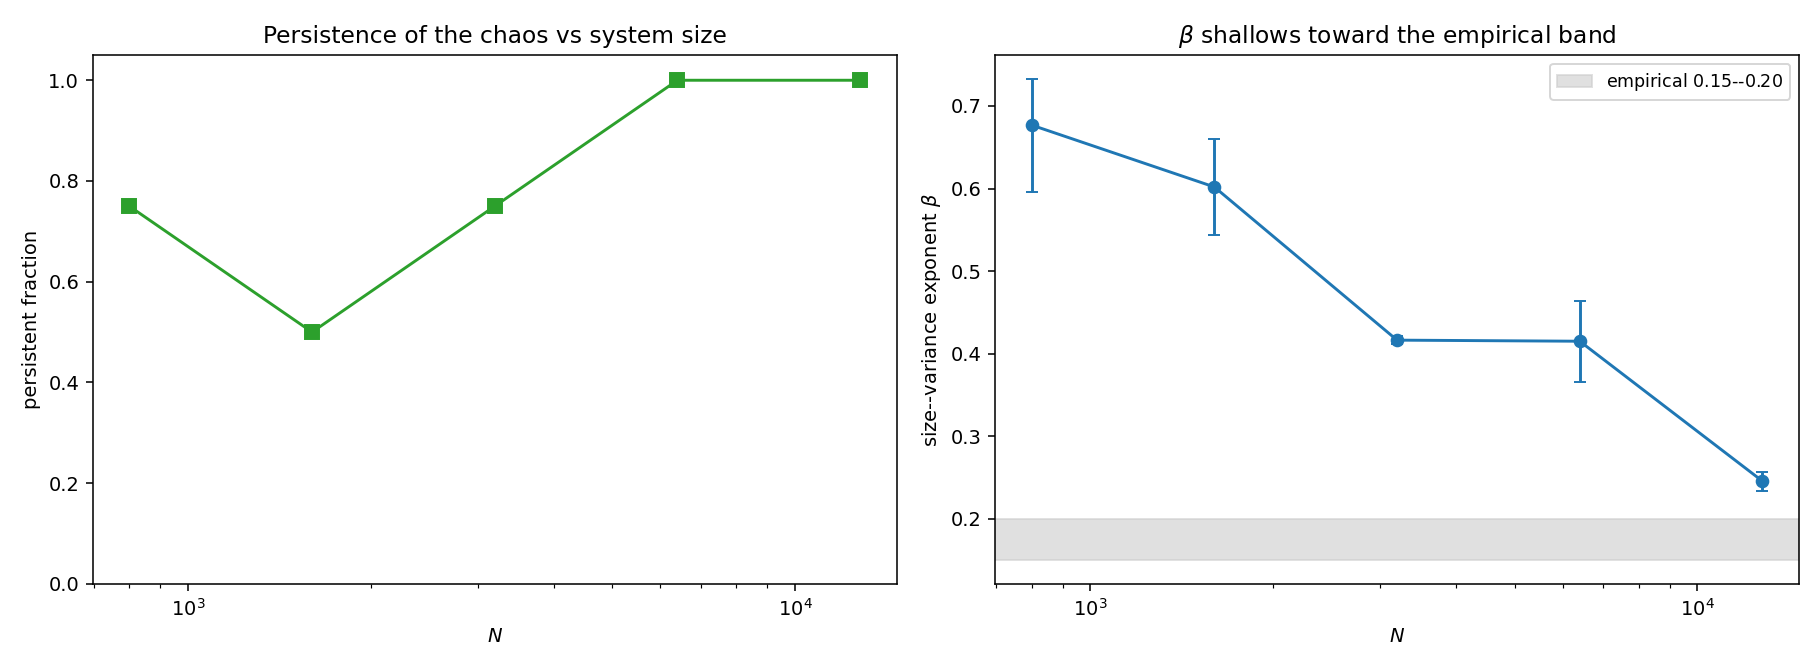
\includegraphics[width=\linewidth]{growing_meanfield.png}
    \caption{Approach to the mean-field limit at $\mu = -1.76$, $\sigma = 1.75$,
    $\lambda = 10^{-3}$. Left: the fraction of realizations that stay persistently
    chaotic at long times rises to one by $N \approx 6000$, so the finite-size
    fragility of the fluctuating phase is a finite-$N$ effect. Right: the
    size--variance exponent $\beta$ measured on the surviving firms falls steadily as $N$
    grows, through the empirical band (shaded); its value at a finite economy size is read
    with the empirical listed-firm protocol in the text.}
    \label{fig:growing-meanfield}
\end{figure}

\begin{figure}[htbp]
    \centering
    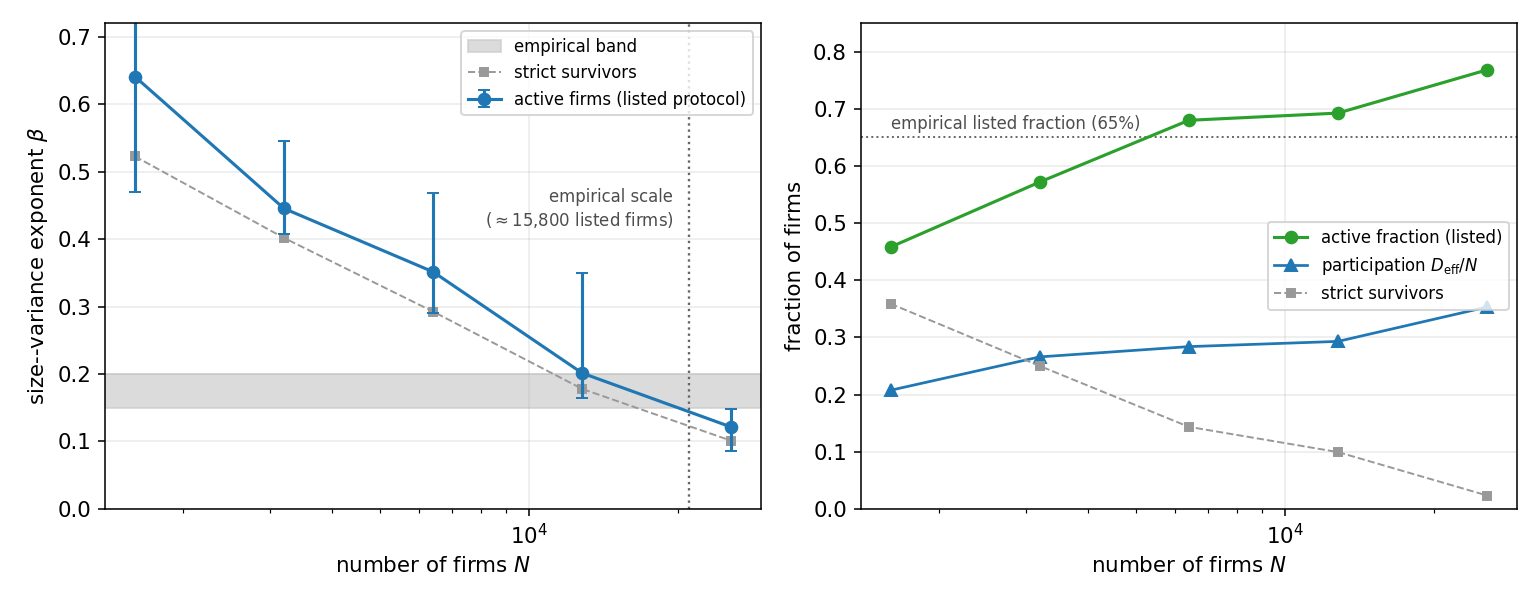
\includegraphics[width=\linewidth]{growing_finite_economy.png}
    \caption{The size--variance exponent and coexistence under the empirical listed-firm
    protocol, at $\mu = -1.76$, $\sigma = 1.75$, $\lambda = 10^{-3}$. A firm is counted
    while its relative size exceeds one per cent of the mean firm and contributes growth
    rates only then, retaining firms with at least twenty rates. Left: the exponent
    $\beta$ falls through the empirical band (shaded) as the economy grows; the dotted line
    marks the economy size at which the number of active firms equals the empirical sample
    of about $15{,}800$ listed firms, where $\beta \approx 0.15$, at the lower edge of the
    band. The strict never-delisted survivors (dashed) give a slightly lower exponent, the
    calm-subsample selection bias. Right: coexistence is extensive, the active fraction and
    the participation ratio $D_{\mathrm{eff}}/N$ both roughly flat in $N$ and near the
    empirical listed fraction, while the strict survivor count (dashed) falls only because
    its fixed share floor becomes a stiffer cutoff as the mean share shrinks. Error bars
    are the interquartile spread over graph realizations.}
    \label{fig:growing-finite-economy}
\end{figure}

Under the own-degree normalization each firm's couplings are scaled by its own degree, so
that every firm carries a disorder field of the same variance whatever its connectivity,
the natural per-fan-in scaling on a heterogeneous graph. The exponent is then a clean
power law that is robust across system size, a genuine thermodynamic quantity, but its
value is steeper, $\beta \approx 0.7$, about three times the empirical one. The two normalizations therefore trade against each other on
magnitude: the mean-degree one reaches the empirical value at the empirical economy size,
the own-degree one fixes a size-independent exponent that is too steep. The difference is
the hubs, which the mean-degree normalization over-couples, a node accumulating a disorder
field that grows with its degree, and which the own-degree normalization quiets to a
common one. Magnitude, however, is not where the granular models fail.

\section{Higher moments and the multiscaling}
\label{sec:growing-multiscaling}

The size--variance exponent is only the first moment of a richer object, the distribution
of growth volatility conditional on size, and it is on the higher moments that the
granular models break. \citet{moran2024} show that the $q$-th moment of the
size-conditioned volatility decays as a power law, $E[\sigma^q \mid S] \sim S^{-\zeta_q}$,
but with an exponent that depends on the order $q$: in the data
$\zeta_1,\dots,\zeta_4 \approx 0.20,\,0.39,\,0.51,\,0.58$, rising with $q$. A granular
composition of independent sub-units predicts the opposite, an exponent independent of
$q$, so this multiscaling is the observable the granular picture cannot reproduce, and the
one \citet{moran2024} read as the fingerprint of correlations that grow with firm size.

The own-degree relative GLV reproduces it. Figure~\ref{fig:growing-multiscaling} measures
the first four moments of the size-conditioned volatility in the model and fits each on
its decline branch. The exponents rise with the order,
$\zeta_1,\dots,\zeta_4 \approx 0.67,\,1.26,\,1.73,\,2.06$; their overall scale is the
steep one of the own-degree normalization, but once divided by $\zeta_1$ the
$q$-dependence, $1,\,1.9,\,2.6,\,3.1$, lies almost on top of the empirical
$1,\,2.0,\,2.6,\,2.9$ and far from the flat granular prediction (right panel). The model
produces the same anomalous scaling of the higher moments as the data, with no internal
firm structure and nothing put in by hand: the size-growing correlations the granular
picture must assume are generated here by the interactions.

The mean-degree normalization fails this test, and instructively. Its over-coupled hubs
give the largest firms a heavy-tailed volatility, so the higher moments are dominated by a
volatile minority and rise with size rather than falling; the measured $\zeta_q$ decrease
with $q$ and turn negative by $q = 4$, the opposite of the data. The discriminating
observable thus picks out the own-degree normalization, the one that quiets the hubs into
the thin-tailed volatility distribution the data show.

\begin{figure}[htbp]
    \centering
    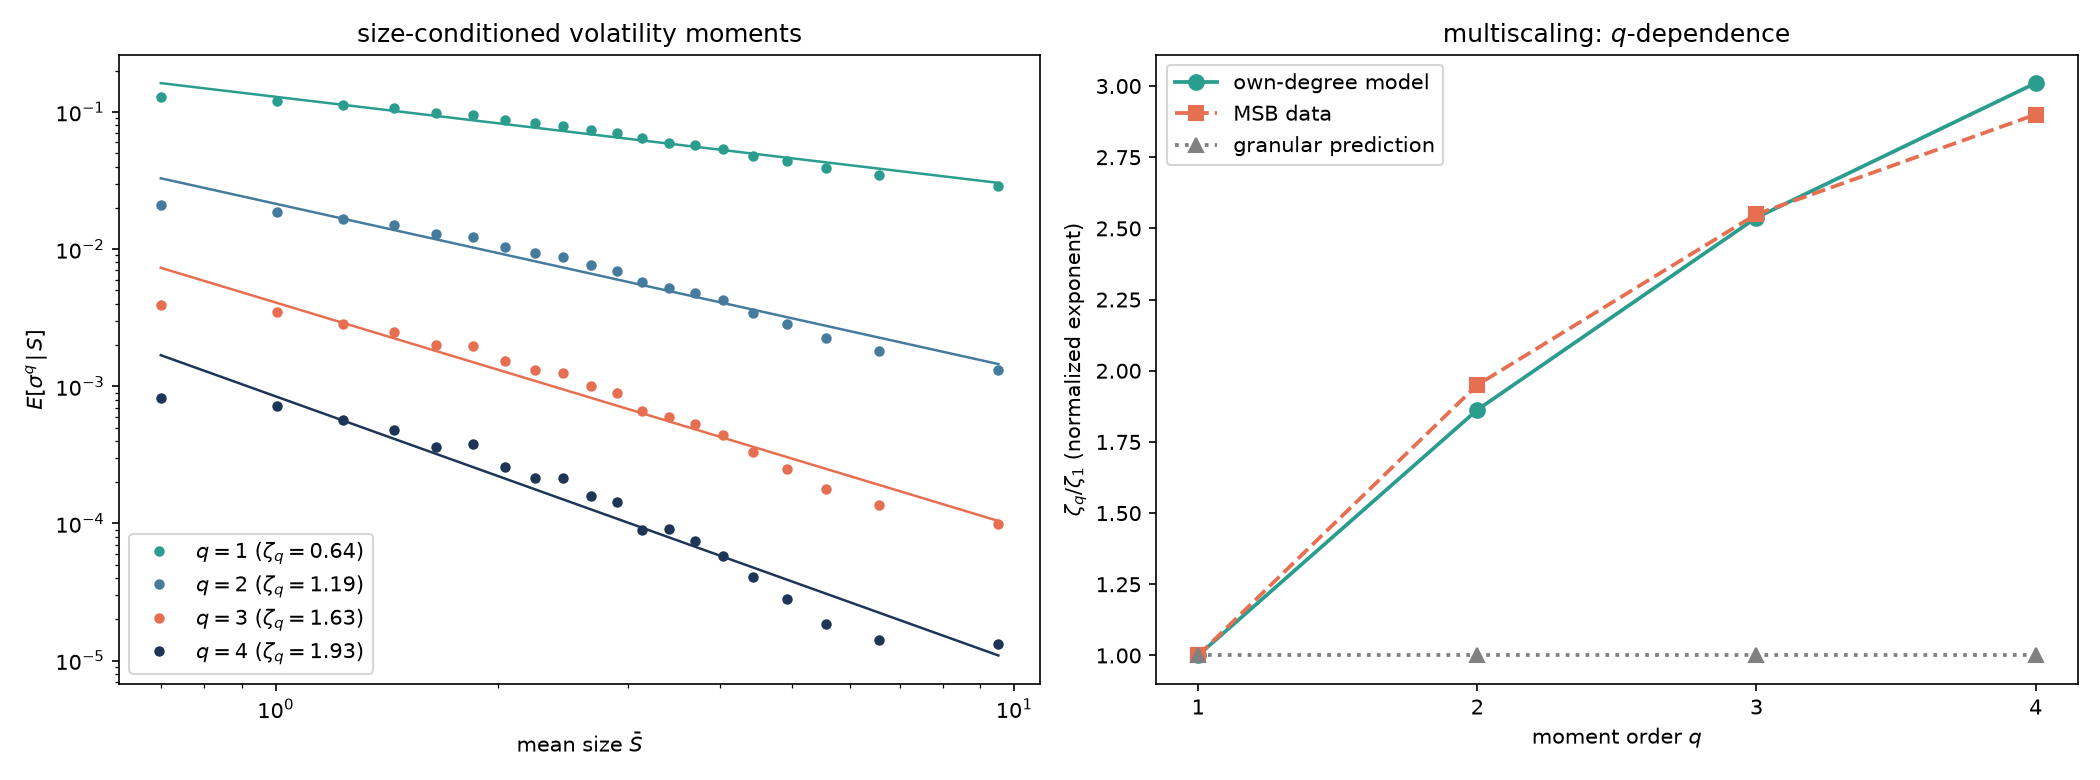
\includegraphics[width=\linewidth]{growing_multiscaling.png}
    \caption{Multiscaling of the size-conditioned volatility in the own-degree model,
    $\mu = -1.76$, $\sigma = 1.75$. Left: the first four moments $E[\sigma^q \mid S]$
    against mean size on a double-logarithmic scale, each fitted on its decline branch;
    the slopes steepen with the order $q$, giving exponents
    $\zeta_1,\dots,\zeta_4 \approx 0.67,\,1.26,\,1.73,\,2.06$. Right: the exponents
    normalized by the first, $\zeta_q/\zeta_1$, against the moment order, for the model,
    the data of \citet{moran2024}, and the granular prediction of a $q$-independent
    exponent. The model reproduces the empirical $q$-dependence and refutes the granular
    one; only the overall scale differs, the own-degree exponent being about three times
    the empirical.}
    \label{fig:growing-multiscaling}
\end{figure}

The multiscaling is one of three size-conditioned tests by which \citet{moran2024}
separate the data from the granular models, and the own-degree relative GLV passes the
other two as well (Fig.~\ref{fig:growing-conditional}). The first is a collapse: rescaled
by its size-conditional mean, the per-firm volatility distribution $\sigma_i/\bar\sigma(S)$
is the same at every size, with a bounded tail, as in the data. The second is the sharper.
Were a firm an aggregate of many independent parts, the central limit theorem would drive
its growth distribution toward a Gaussian as it grew, the excess kurtosis falling to zero
with size; the data do the opposite, large firms remaining at least as fat-tailed as small
ones. The model reproduces this anti-Gaussian trend, the excess kurtosis of the
size-unmixed growth rising from about three for the smallest firms to ten for the largest,
the signature that a firm's growth is not a sum of independent contributions but carries
the correlations the interactions impose. The model thus clears not only the
size--variance exponent that the granular models also fit, but every conditional test by
which the data reject them.

\begin{figure}[htbp]
    \centering
    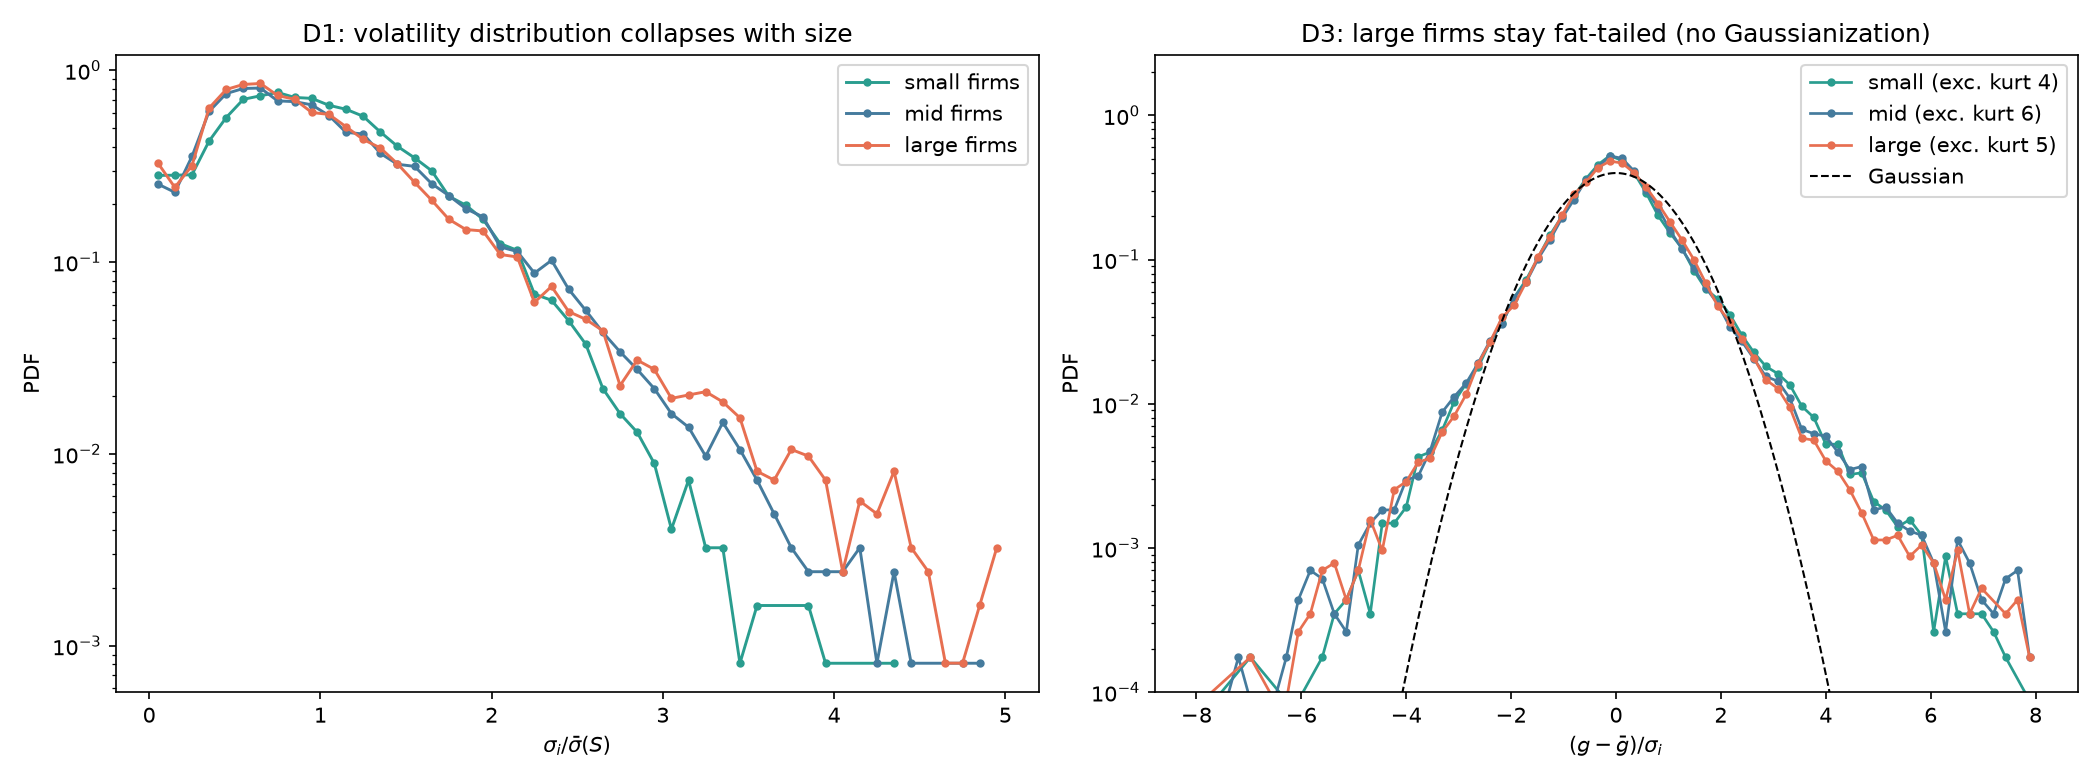
\includegraphics[width=\linewidth]{growing_conditional.png}
    \caption{The other two discriminating tests of \citet{moran2024}, on the own-degree
    model. Left (D1): the per-firm volatility distribution, rescaled by its
    size-conditional mean $\sigma_i/\bar\sigma(S)$, collapses onto a single size-independent
    shape with a bounded tail. Right (D3): the size-unmixed growth $(g-\bar g)/\sigma_i$
    stays fat-tailed at every size, well above the Gaussian, and the largest firms are the
    fattest, the excess kurtosis rising from about three to ten with size, rather than
    approaching a Gaussian as an aggregate of independent parts would.}
    \label{fig:growing-conditional}
\end{figure}

The dependence on the normalization is itself informative, and it shows that the gap in
magnitude cannot be closed within this family without losing the structure. Writing the
noise scaling as $\sigma/k_i^{\,p}$, with $p = 0$ the mean-degree normalization and
$p = \tfrac12$ the own-degree one, sweeps the hub loudness continuously, and with it both
the exponent and its higher moments (Fig.~\ref{fig:growing-normalization}). The
first-moment exponent rises monotonically with $p$, from about $0.15$ at $p = 0$ to $0.69$
at $p = \tfrac12$, and reaches the empirical band only at $p = 0$. The multiscaling matches
the data only at the other end, $p \gtrsim 0.4$, where $\beta$ is two to three times too
steep; as $p$ falls and $\beta$ comes down the higher-moment exponents flatten, and by
$p = 0$ they invert, the moments rising with size rather than falling. The two never
coincide. The hub-quieting that produces the thin-tailed multiscaling is the same that
over-stabilizes the largest firms, so bringing $\beta$ into the band requires loud hubs,
which destroy the structure. Magnitude and multiscaling are two faces of one parameter,
and no normalization in this family yields both at once. The gap is therefore not a matter
of calibration but of a missing ingredient, the size-dependent correlations of a firm
built from many parts, which the single-level model cannot supply.

\begin{figure}[htbp]
    \centering
    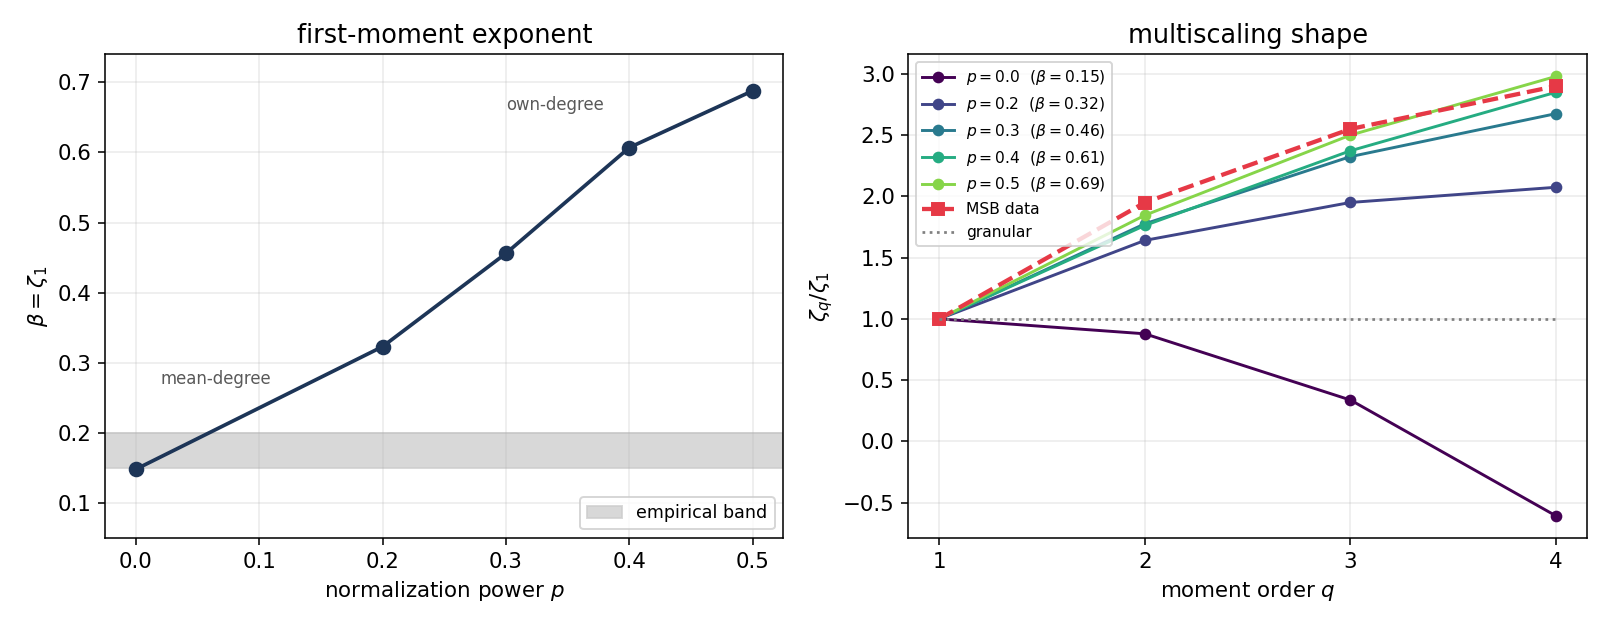
\includegraphics[width=\linewidth]{growing_normalization.png}
    \caption{The magnitude--structure trade-off across the normalization family, the noise
    scaled as $\sigma/k_i^{\,p}$, at $\mu = -1.76$, $\sigma = 1.75$, $N = 1.3\times10^4$;
    $p = 0$ is the mean-degree normalization and $p = \tfrac12$ the own-degree one. Left:
    the first-moment exponent $\beta = \zeta_1$ rises monotonically with $p$ and enters the
    empirical band (shaded) only at $p = 0$. Right: the normalized higher-moment exponents
    $\zeta_q/\zeta_1$ match the data of \citet{moran2024} only for $p \gtrsim 0.4$, where
    $\beta$ is far too steep, and collapse, inverting by the fourth moment, at the $p = 0$
    where $\beta$ lies in the band. No single $p$ reproduces both the magnitude and the
    multiscaling.}
    \label{fig:growing-normalization}
\end{figure}

\section{The role of the interactions}
\label{sec:growing-ablation}

The model carries no external heterogeneity and no explicit noise: the only source of
fluctuation is the disordered interaction matrix. To confirm that the firm-growth
statistics are produced by the interactions, and are not an artifact of the
multiplicative structure or the immigration floor, we switch the disorder off and dial
it back up. Table~\ref{tab:growing-ablation} sweeps $\sigma$ at fixed $\mu$, $\lambda$
and $N$. Below the threshold $\sigma_c = \sqrt{2}$ the dynamics freeze: the late-time
growth fluctuations are zero to the precision quoted, the shape has relaxed to a fixed
point, and there is no fluctuating state to measure. The persistent fluctuations and
the fat-tailed tent appear only once $\sigma$ crosses $\sigma_c$, growing with the
disorder. With no noise in the model, the fluctuations can come only from the disorder,
and removing it removes them entirely.

\begin{table}[h]
    \centering
    \begin{tabular}{rccc}
        \hline
        $\sigma$ & growth fluctuation & excess kurtosis & fat-tailed tent? \\
        \hline
        $0.00$ & $0.000$ & --   & no  \\
        $0.50$ & $0.000$ & --   & no  \\
        $1.00$ & $0.000$ & --   & no  \\
        $1.41$ & $0.000$ & --   & no  \\
        $1.60$ & $0.085$ & $14$ & yes \\
        $1.75$ & $0.175$ & $14$ & yes \\
        \hline
    \end{tabular}
    \caption{Disorder ablation at $\mu = -1.76$, $\lambda = 10^{-3}$, $N = 3200$ on a
    power-law graph. ``Growth fluctuation'' is the standard deviation of the pooled
    late-window growth rates. Below the chaotic threshold $\sigma_c = \sqrt{2}$ the state
    freezes (growth fluctuation zero to the precision quoted) and there is no genuine
    fluctuating distribution to characterize, so the kurtosis is left blank; the
    persistent fluctuations and the fat-tailed tent switch on only once $\sigma$ crosses
    $\sigma_c$. (A nonzero $\beta$ can still be fitted below threshold, but on a frozen
    state during its relaxation, the V transient of Appendix~\ref{chap:results}, not on a
    stationary fluctuating law.)}
    \label{tab:growing-ablation}
\end{table}

This is the distinction the introduction asked for. The firm-growth statistics here are
a between-firm effect, generated by the network of interactions, and not a within-firm
one: with the interactions removed there is nothing left, no noise carrying the
fluctuations and no single-firm mechanism producing a tail. It is also the size of the
result that separates this model from the simplest alternatives. A growing economy with
a stationary heavy-tailed size distribution can be had from a mean-field multiplicative
model with injected noise \citep{bouchaudmezard2000}, but there the fluctuations are put
in by hand and there is no network. Here the same growing aggregate, the heavy tails,
and the slow size--variance decay arise together from a single ingredient, the disordered
interactions, which is the size-dependent correlation mechanism \citet{moran2024}
identify as the one the granular models lack.

\section{Discussion}
\label{sec:growing-discussion}

This chapter closes the gap left by Appendix~\ref{chap:results}. Making the
Lotka--Volterra interactions relative to the mean firm turns the finite-time divergence
of the standard model into steady exponential growth, and in the disordered regime
$\sigma > \sigma_c$ the resulting economy grows while its composition fluctuates without
ever settling. In this genuinely nonstationary state the size--variance relation is a
stationary law that falls with the empirical sign; it clears the conditional tests by
which the data reject the granular models, the anomalous multiscaling of its higher
moments and the persistence of fat tails in the largest firms; the growth-rate
distribution is symmetric and fat-tailed; and switching off the disorder removes them all,
placing their origin in the interactions.

Three honest qualifications bound the claim. The model itself is not new: it is the
disordered replicator equation \citep{diederich1989,hofbauer81}, equivalently the
chaotic phase of the disordered Lotka--Volterra model \citep{bunin2017,galla2018,roy2020},
and its finite-size fragility and approach to a robust mean-field fluctuating phase are
known features of that system. What is specific here is the use of this state, on a
heterogeneous graph and with the interactions made relative so that the aggregate grows,
as a model of firm growth, and the finding that its firm-growth statistics match the
empirical ones. The exponent's magnitude, second, is matched only up to the
normalization of the couplings: with the own-degree scaling it is a clean thermodynamic
power law but about three times too steep, while with the mean-degree scaling it reaches
the empirical value at the observed economy size of order $10^4$ listed firms but does not
settle to a thermodynamic constant. It is the order-dependence of the higher moments, not
the magnitude of the first, that the model reproduces and the granular picture does not.
Third, the economy grows in the large
majority of realizations rather than in every one, the operating point sitting in the
growing band but not far from its $g_{\mathrm{eff}} = 0$ boundary. Beyond these, what the model adds that the granular picture cannot is the multiscaling of
the higher moments, the signature \citet{moran2024} read as correlations that grow with
firm size; measuring that correlation structure directly,
rather than through its moments, and closing the factor of three in the exponent's
magnitude, which we have shown no normalization in this family can do, are the natural
next steps, both pointing to the same missing ingredient, a firm built from many
correlated parts.
